\documentclass[a4paper,12pt,oneside]{book}
\usepackage[utf8]{inputenc}
\usepackage{amssymb}
\usepackage{amsmath}
\usepackage{graphicx}
\graphicspath{ {images/} }
\usepackage{times}
\usepackage{geometry}
\usepackage{setspace}
\usepackage{tocloft}
\usepackage{tabu}
\usepackage{fancyhdr}
\usepackage{tabularx}

%Defining some new commands for some repeated text.
%Modify your name and other details in this section.
\newcommand{\theauthor}{John Smith}
\newcommand{\therollno}{314159265}
\newcommand{\thedegree}{B.Tech}
\newcommand{\thedegreelong}{Bachelor of Technology}
\newcommand{\thetitle}{Absurdly long Thesis Title Written in All Caps}
\newcommand{\theguide}{Name of Guide}
\newcommand{\thehod}{Name of HOD}
\newcommand{\thedepartment}{Name of the Department}
\newcommand{\theyear}{2016}
\newcommand{\theacadyear}{2015-2016}
\newcommand{\themonth}{May}

%Set paragraph indentation to zero
\setlength\parindent{0pt}
%Set paragraph spacing
\setlength{\parskip}{12pt}

%Set the paper size and the margins
\geometry{a4paper, tmargin=1in, rmargin=1in, bmargin=1in, lmargin=1.5in}
\usepackage{titlesec}
\usepackage[hidelinks]{hyperref}

%Format the chapter headings to be 14pt, centered and Uppercase
\titleformat{\chapter}[display]
  {\large\bfseries\centering}
  {\MakeUppercase\chaptertitlename\ \thechapter}{7pt}{\large\MakeUppercase}

%Format the section headings to be uppercase and 12pt
\titleformat{\section}[hang]
  {\MakeUppercase\normalfont\bfseries}
  {\thesection}{12pt}{\MakeUppercase}

%Format the subsections to be 12pt
\titleformat{\subsection}[hang]
  {\MakeUppercase\normalfont\bfseries}
  {\thesubsection}{12pt}{}

%Set the spacing between the chapter headings and the margins
\titlespacing*{\chapter}{0pt}{0pt}{24pt}
\titlespacing*{\section}{0pt}{0pt}{0pt}
\titlespacing*{\subsection}{0pt}{0pt}{0pt}
%Add dots to the table of contents for chapters
\renewcommand{\cftchapleader}{\cftdotfill{\cftdotsep}} % for chapters
%Set the spacings before and after the titles for the TOC, LOF and LOT
\setlength{\cftbeforetoctitleskip}{0.43in}
\setlength{\cftaftertoctitleskip}{21pt}
\setlength{\cftbeforelottitleskip}{0.43in}
\setlength{\cftafterlottitleskip}{21pt}
\setlength{\cftbeforeloftitleskip}{0.43in}
\setlength{\cftafterloftitleskip}{21pt}
%Set the fontsize and formatting for the TOC, LOF and LOT 
\renewcommand\contentsname{\centerline{\fontsize{16pt}{16pt}\selectfont TABLE OF CONTENTS}}
\renewcommand\listfigurename{\centerline{\fontsize{16pt}{16pt}\selectfont LIST OF FIGURES}}
\renewcommand\listtablename{\centerline{\fontsize{16pt}{16pt}\selectfont LIST OF TABLES}}
%Setting page numbers to bottom center
\pagestyle{fancy}
\cfoot{\thepage}
\rhead{}
\lhead{}
\renewcommand{\headrulewidth}{0pt}
\renewcommand{\footrulewidth}{0pt}
%Setting bibliography title format
\renewcommand{\bibname}{\fontsize{16pt}{24pt}\selectfont References \hfill}


\begin{document}
%Adding all the stuff that should be numbered with roman numerals
\frontmatter
\addtocontents{toc}{\textbf{Title}\hfill\textbf{Page No.}\par}
\addtocontents{toc}{\vspace{-0.3cm}}
\begin{titlepage}
\begin{center}
\fontsize{18pt}{1cm}\selectfont \textbf{ABSURDLY LONG THESIS TITLE THAT HAS TO BE WRITTEN IN ALL CAPS}

\vspace*{1.4cm}
\fontsize{14pt}{21pt}\selectfont A thesis submitted in partial fulfillment of the requirements for\\
the award of the degree of

\vspace*{0.8cm}
\fontsize{14pt}{1cm}\selectfont\textbf{B.Tech} 

\vspace*{0.8cm}
\textbf{in\\DEPARTMENT NAME HERE}

\vspace*{2.0cm}
By

\textbf{NAME (ROLL NO.)}

\vspace*{3.4cm}

\includegraphics[width=1.25in]{NITT-Logo}

\vspace*{0.3cm}
\fontsize{16pt}{16pt}\selectfont \textbf{METALLURGICAL AND MATERIALS ENGINEERING\\NATIONAL INSTITUTE OF TECHNOLOGY\\TIRUCHIRAPPALLI-620015}

\vspace*{0.5cm}
\textbf{MAY 2016}
\end{center}
\end{titlepage}

\thispagestyle{plain}
\begin{center}
\textbf{BONAFIDE CERTIFICATE}
\end{center}

\vspace{0.3cm}
\fontsize{12pt}{18pt}\selectfont This is to certify that the project titled \textbf{ABSURDLY LONG THESIS TITLE THAT YOU HAVE TO WRITE IN ALL CAPS} is a bonafide record of the work done by
\vspace{0.3cm}

\begin{center}
\textbf{Name (Roll No.)}
\end{center}

\vspace{0.3cm}
\noindent
\fontsize{12pt}{18pt}\selectfont in partial fulfillment of the requirements for the award of the degree of \textbf{Bachelor of Technology} in \textbf{Metallurgical and Materials Engineering} of the \textbf{NATIONAL INSTITUTE OF TECHNOLOGY, TIRUCHIRAPPALLI}, during the year 2015-2016.

\vspace{3cm}

\begin{tabu} to \textwidth { X[l] X[c] }

 \textbf{Dr. S. NATARAJAN} & \textbf{Dr. S. P. KUMARESH BABU} \\ \hspace{1cm} Guide & Head of the Department

\end{tabu}

\vspace{4cm}
Project Viva-voce held on \rule{5.5cm}{.1pt}

\vspace{4cm}
\textbf{Internal Examiner} \hfill \textbf{External Examiner}

\newpage

\addcontentsline{toc}{chapter}{ABSTRACT}
\addtocontents{toc}{\vspace{-0.3cm}}
\thispagestyle{plain}
\begin{center}
\textbf{\textbf{\fontsize{16pt}{24pt}\selectfont ABSTRACT}}
\end{center}

\vspace{0.3cm}
\fontsize{12pt}{18pt}\selectfont Removal of colour from industrial wastewater can be achieved by extraction using liquid
emulsion membrane. A dye, named, Crystal Violet (CV) is extracted using water/oil/water
liquid emulsion membrane. An experiment on single dye component is carried out. A stable
emulsion is formed by agitating NaOH solution and an organic solvent (n-hexane) at high
speed. Span 80 (surfactant) is used to stabilize the membrane. Extraction is carried out by
dispersing the emulsion in an external water phase (feed) at lower speed resulting in the
formation of small globules thereby increasing surface area and providing better extraction.
The constituent (dye) to be extracted from the external phase diffuses through the membrane
phase into the internal phase (NaOH solution). Reaction occurs in the internal phase resulting
in the formation of sodium salt of the dye (s). The emulsion can be reused after
demulsification. During extraction, the effect of Span 80, NaOH concentration, n-hexane,
stirring speed and feed concentration have been investigated. The main objective of this study
is to find the optimum operating conditions for the extraction of crystal violet. 

\textit{Keywords}: Emulsion; Internal phase; Extraction; Diffusion; Dye separation

\newpage

\addcontentsline{toc}{chapter}{ACKNOWLEDGEMENTS}
\addtocontents{toc}{\vspace{-0.3cm}}
\thispagestyle{plain}
\begin{center}
\textbf{\textbf{\fontsize{16pt}{24pt}\selectfont ACKNOWLEDGEMENTS}}
\end{center}

Add the ack text here.

\newpage

\addcontentsline{toc}{chapter}{TABLE OF CONTENTS}
\addtocontents{toc}{\vspace{-0.3cm}}
\tableofcontents
\newpage
\addcontentsline{toc}{chapter}{LIST OF TABLES}
\addtocontents{toc}{\vspace{-0.3cm}}
\listoftables
\newpage
\addcontentsline{toc}{chapter}{LIST OF FIGURES}
\addtocontents{toc}{\vspace{-0.3cm}}
\listoffigures
 
\mainmatter

\chapter{Introduction}
\fontsize{12pt}{18pt}\selectfont
Lorems ipsum dolor sit amet, consectetur adipiscing elit. Vivamus at pulvinar nisi. Phasellus hendrerit, diam placerat interdum iaculis, mauris justo cursus risus, in viverra purus eros at ligula. Ut metus justo, consequat a tristique posuere, laoreet nec nibh. Etiam et scelerisque mauris. Phasellus vel massa magna. Ut non neque id tortor pharetra bibendum vitae sit amet nisi. Duis nec quam quam, sed euismod justo. Pellentesque eu tellus vitae ante tempus malesuada. Nunc accumsan, quam in congue consequat, lectus lectus dapibus erat, id aliquet urna neque at massa. Nulla facilisi. Morbi ullamcorper eleifend posuere. Donec libero leo, faucibus nec bibendum at, mattis et urna. Proin consectetur, nunc ut imperdiet lobortis, magna neque tincidunt lectus, id iaculis nisi justo id nibh. Pellentesque vels sem in erat vulputate faucibus molestie ut lorem\cite{graves2013speech}.

\begin{figure}
    \centering
    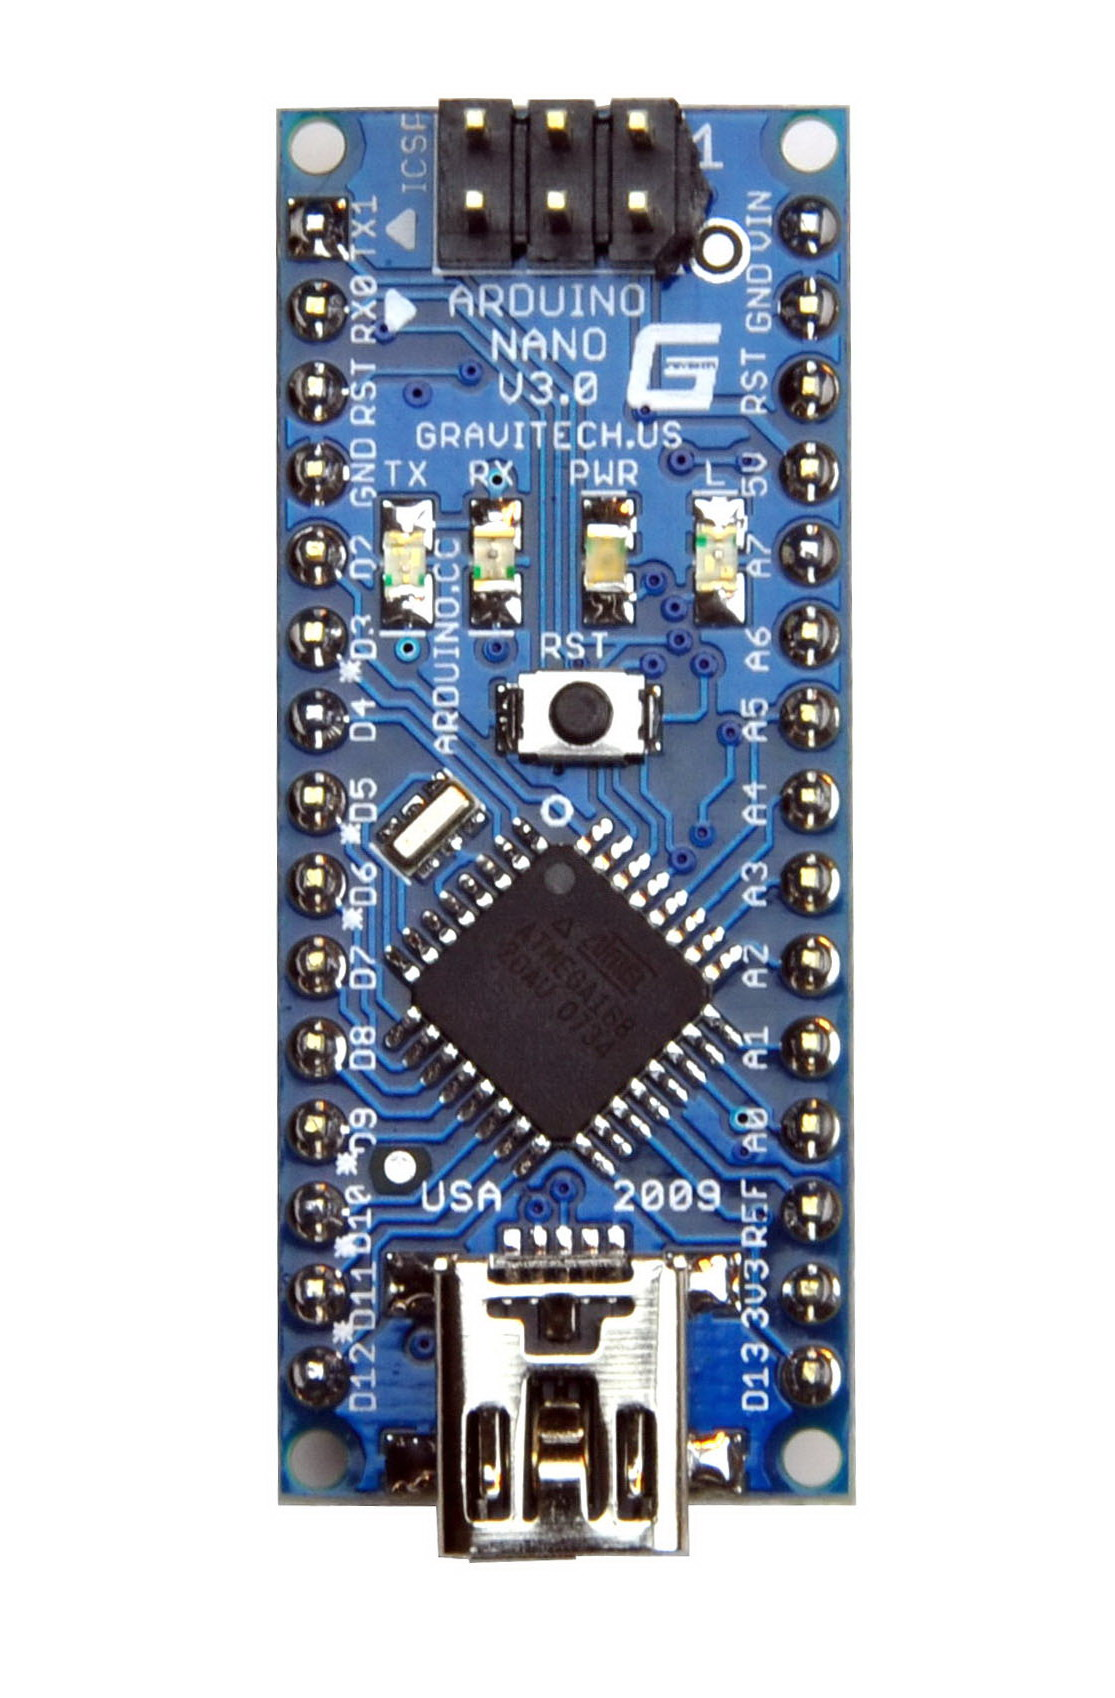
\includegraphics[width=0.5\textwidth, angle=-90]{nano}
    \caption{This is Arduino Nano}
    \label{fig:nano}
\end{figure}

\section{A Section}

Quisque tristique urna in lorem laoreet at laoreet quam congue. Donec dolor turpis, blandit non imperdiet aliquet, blandit et felis. In lorem nisi, pretium sit amet vestibulum sed, tempus et sem. Proin non ante turpis. Nulla imperdiet fringilla convallis. Vivamus vel bibendum nisl. Pellentesque justo lectus, molestie vel luctus sed, lobortis in libero. Nulla facilisi. Aliquam erat volutpat. Suspendisse vitae nunc nunc. Sed aliquet est suscipit sapien rhoncus non adipiscing nibh consequat. Aliquam metus urna, faucibus eu vulputate non, luctus eu justo \cite{wang2002hot}.

\subsection{A Subsection}

Donec urna leo, vulputate vitae porta eu, vehicula blandit libero. Phasellus eget massa et leo condimentum mollis. Nullam molestie, justo at pellentesque vulputate, sapien velit ornare diam, nec gravida lacus augue non diam. Integer mattis lacus id libero ultrices sit amet mollis neque molestie. Integer ut leo eget mi volutpat congue. Vivamus sodales, turpis id venenatis placerat, tellus purus adipiscing magna, eu aliquam nibh dolor id nibh. Pellentesque habitant morbi tristique senectus et netus et malesuada fames ac turpis egestas. Sed cursus convallis quam nec vehicula. Sed vulputate neque eget odio fringilla ac sodales urna feugiat.

Table \ref{table:1} is really awesome and I like it.

The table \ref{table:1} is an example of referenced \LaTeX elements.
 
\begin{table}[h!]
\centering
\caption{Table to test captions and labels}
\begin{tabular}{||c c c c||} 
 \hline
 Col1 & Col2 & Col2 & Col3 \\ [0.5ex] 
 \hline\hline
 1 & 6 & 87837 & 787 \\ 
 2 & 7 & 78 & 5415 \\
 3 & 545 & 778 & 7507 \\
 4 & 545 & 18744 & 7560 \\
 5 & 88 & 788 & 6344 \\ [1ex] 
 \hline
\end{tabular}
\label{table:1}
\end{table}

\section{Another Section}

Phasellus nisi quam, volutpat non ullamcorper eget, congue fringilla leo. Cras et erat et nibh placerat commodo id ornare est. Nulla facilisi. Aenean pulvinar scelerisque eros eget interdum. Nunc pulvinar magna ut felis varius in hendrerit dolor accumsan. Nunc pellentesque magna quis magna bibendum non laoreet erat tincidunt. Nulla facilisi.

Duis eget massa sem, gravida interdum ipsum. Nulla nunc nisl, hendrerit sit amet commodo vel, varius id tellus. Lorem ipsum dolor sit amet, consectetur adipiscing elit. Nunc ac dolor est. Suspendisse ultrices tincidunt metus eget accumsan. Nullam facilisis, justo vitae convallis sollicitudin, eros augue malesuada metus, nec sagittis diam nibh ut sapien. Duis blandit lectus vitae lorem aliquam nec euismod nisi volutpat. Vestibulum ornare dictum tortor, at faucibus justo tempor non. Nulla facilisi. Cras non massa nunc, eget euismod purus. Nunc metus ipsum, euismod a consectetur vel, hendrerit nec nunc.

\begin{figure}
    \centering
    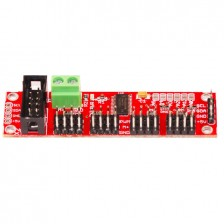
\includegraphics{servo_driver}
    \caption{This is a servo controller.}
    \label{fig:servo_driver}
\end{figure}

Single equation
\begin{equation}
    e^{i\pi} = -1
\end{equation}

Multiple equations
\begin{align}
\textnormal{State Vector: }& x = \begin{bmatrix}q&\vec{\omega}\end{bmatrix}^T \\
\textnormal{Process Model: }& x_{k+1} = A(x_k, w_k) = \begin{bmatrix}q_kq_wq_{\Delta}\\\omega_{k}\end{bmatrix}\\
\textnormal{Measurement Model: }& z_k = H(x_k, v_k) = \begin{bmatrix}q_kgq_k^* + \vec{v}_{acc}\\\vec{\omega}_k + \vec{v}_{rot}\end{bmatrix}
\end{align}

This is an example of how you can reference an image. This sentence is referring to the Figure \ref{fig:tree}

\begin{figure}
    \centering
    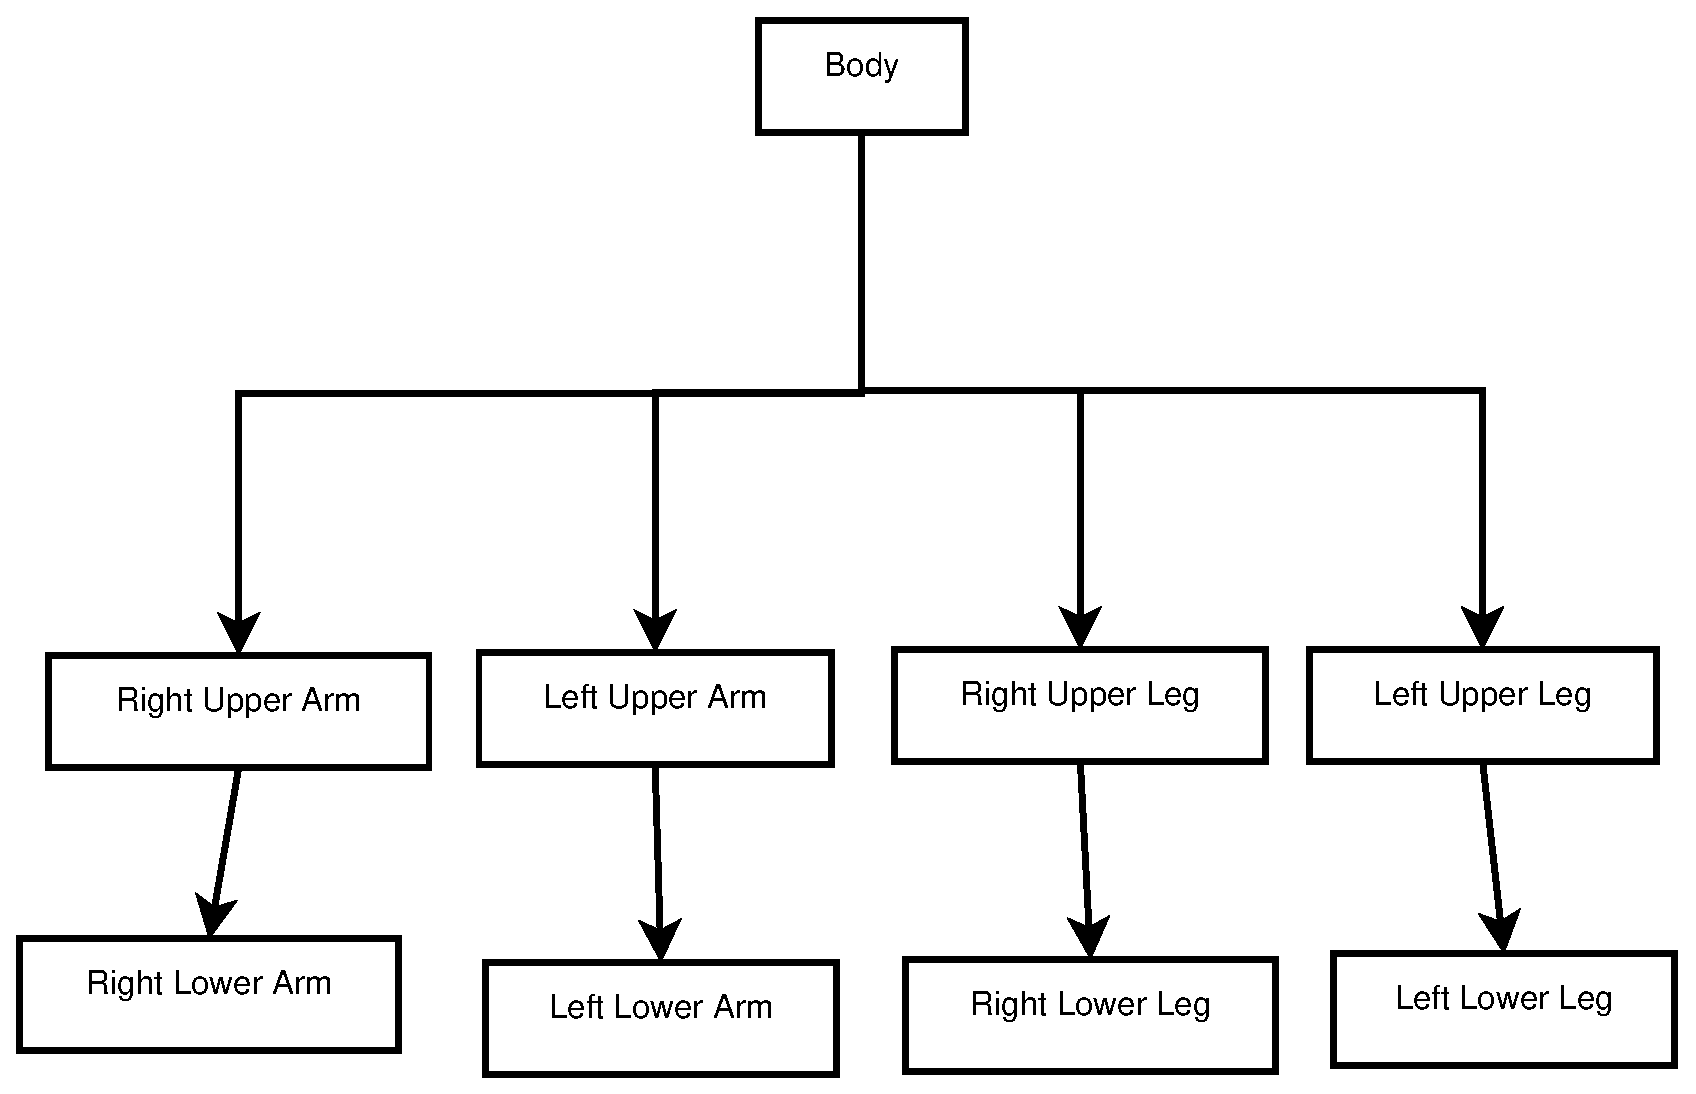
\includegraphics[width=\textwidth]{KinematicTree}
    \caption{This is some awesome thing.}
    \label{fig:tree}
\end{figure}


\chapter{Implementation}
\fontsize{12pt}{18pt}\selectfont
Lorem ipsum dolor sit amet, consectetur adipiscing elit. Vivamus at pulvinar nisi. Phasellus hendrerit, diam placerat interdum iaculis, mauris justo cursus risus, in viverra purus eros at ligula. Ut metus justo, consequat a tristique posuere, laoreet nec nibh. Etiam et scelerisque mauris. Phasellus vel massa magna. Ut non neque id tortor pharetra bibendum vitae sit amet nisi. Duis nec quam quam, sed euismod justo. Pellentesque eu tellus vitae ante tempus malesuada. Nunc accumsan, quam in congue consequat, lectus lectus dapibus erat, id aliquet urna neque at massa. Nulla facilisi. Morbi ullamcorper eleifend posuere. Donec libero leo, faucibus nec bibendum at, mattis et urna. Proin consectetur, nunc ut imperdiet lobortis, magna neque tincidunt lectus, id iaculis nisi justo id nibh. Pellentesque vel sem in erat vulputate faucibus molestie ut lorem\cite{graves2013speech}.

\begin{figure}
    \centering
    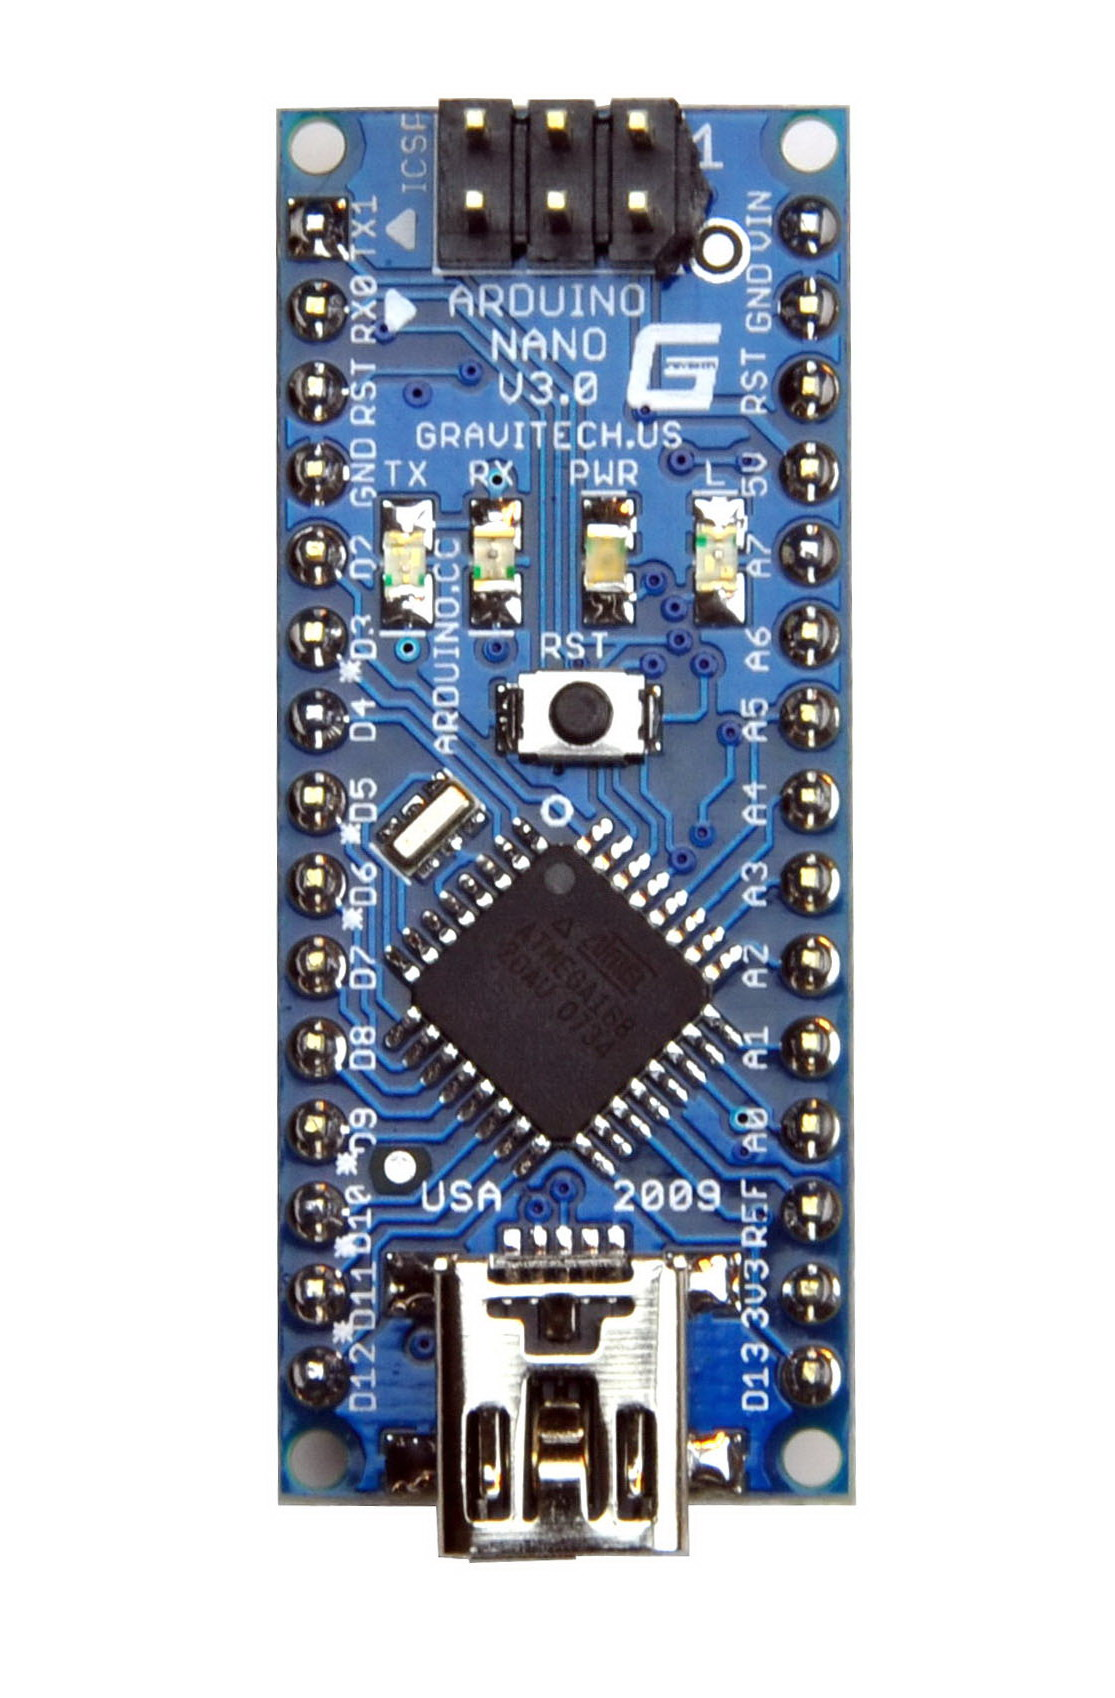
\includegraphics{nano}
    \caption{This is Arduino Nano}
    \label{fig:nano2}
\end{figure}

\section{A Section}

Quisque tristique urna in lorem laoreet at laoreet quam congue. Donec dolor turpis, blandit non imperdiet aliquet, blandit et felis. In lorem nisi, pretium sit amet vestibulum sed, tempus et sem. Proin non ante turpis. Nulla imperdiet fringilla convallis. Vivamus vel bibendum nisl. Pellentesque justo lectus, molestie vel luctus sed, lobortis in libero. Nulla facilisi. Aliquam erat volutpat. Suspendisse vitae nunc nunc. Sed aliquet est suscipit sapien rhoncus non adipiscing nibh consequat. Aliquam metus urna, faucibus eu vulputate non, luctus eu justo \cite{wang2002hot}.

\subsection{A Subsection}

Donec urna leo, vulputate vitae porta eu, vehicula blandit libero. Phasellus eget massa et leo condimentum mollis. Nullam molestie, justo at pellentesque vulputate, sapien velit ornare diam, nec gravida lacus augue non diam. Integer mattis lacus id libero ultrices sit amet mollis neque molestie. Integer ut leo eget mi volutpat congue. Vivamus sodales, turpis id venenatis placerat, tellus purus adipiscing magna, eu aliquam nibh dolor id nibh. Pellentesque habitant morbi tristique senectus et netus et malesuada fames ac turpis egestas. Sed cursus convallis quam nec vehicula. Sed vulputate neque eget odio fringilla ac sodales urna feugiat.

\subsection{B Sub-Section}

Table \ref{table:1} is really awesome and I like it.

The table \ref{table:1} is an example of referenced \LaTeX elements.
 
\begin{table}[h!]
\centering
\begin{tabular}{||c c c c||} 
 \hline
 Col1 & Col2 & Col2 & Col3 \\ [0.5ex] 
 \hline\hline
 1 & 6 & 87837 & 787 \\ 
 2 & 7 & 78 & 5415 \\
 3 & 545 & 778 & 7507 \\
 4 & 545 & 18744 & 7560 \\
 5 & 88 & 788 & 6344 \\ [1ex] 
 \hline
\end{tabular}
\caption{Table to test captions and labels}
\label{table:2}
\end{table}

\section{Another Section}

Phasellus nisi quam, volutpat non ullamcorper eget, congue fringilla leo. Cras et erat et nibh placerat commodo id ornare est. Nulla facilisi. Aenean pulvinar scelerisque eros eget interdum. Nunc pulvinar magna ut felis varius in hendrerit dolor accumsan. Nunc pellentesque magna quis magna bibendum non laoreet erat tincidunt. Nulla facilisi.

Duis eget massa sem, gravida interdum ipsum. Nulla nunc nisl, hendrerit sit amet commodo vel, varius id tellus. Lorem ipsum dolor sit amet, consectetur adipiscing elit. Nunc ac dolor est. Suspendisse ultrices tincidunt metus eget accumsan. Nullam facilisis, justo vitae convallis sollicitudin, eros augue malesuada metus, nec sagittis diam nibh ut sapien. Duis blandit lectus vitae lorem aliquam nec euismod nisi volutpat. Vestibulum ornare dictum tortor, at faucibus justo tempor non. Nulla facilisi. Cras non massa nunc, eget euismod purus. Nunc metus ipsum, euismod a consectetur vel, hendrerit nec nunc.

\begin{figure}
    \centering
    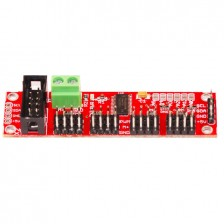
\includegraphics{servo_driver}
    \caption{This is a servo controller.}
    \label{fig:servo_driver2}
\end{figure}

Single equation
\begin{equation}
    e^{i\pi} = -1
\end{equation}

Multiple equations
\begin{align}
\textnormal{State Vector: }& x = \begin{bmatrix}q&\vec{\omega}\end{bmatrix}^T \\
\textnormal{Process Model: }& x_{k+1} = A(x_k, w_k) = \begin{bmatrix}q_kq_wq_{\Delta}\\\omega_{k}\end{bmatrix}\\
\textnormal{Measurement Model: }& z_k = H(x_k, v_k) = \begin{bmatrix}q_kgq_k^* + \vec{v}_{acc}\\\vec{\omega}_k + \vec{v}_{rot}\end{bmatrix}
\end{align}

This is an example of how you can reference an image. This sentence is referring to the Figure \ref{fig:tree}

\begin{figure}
    \centering
    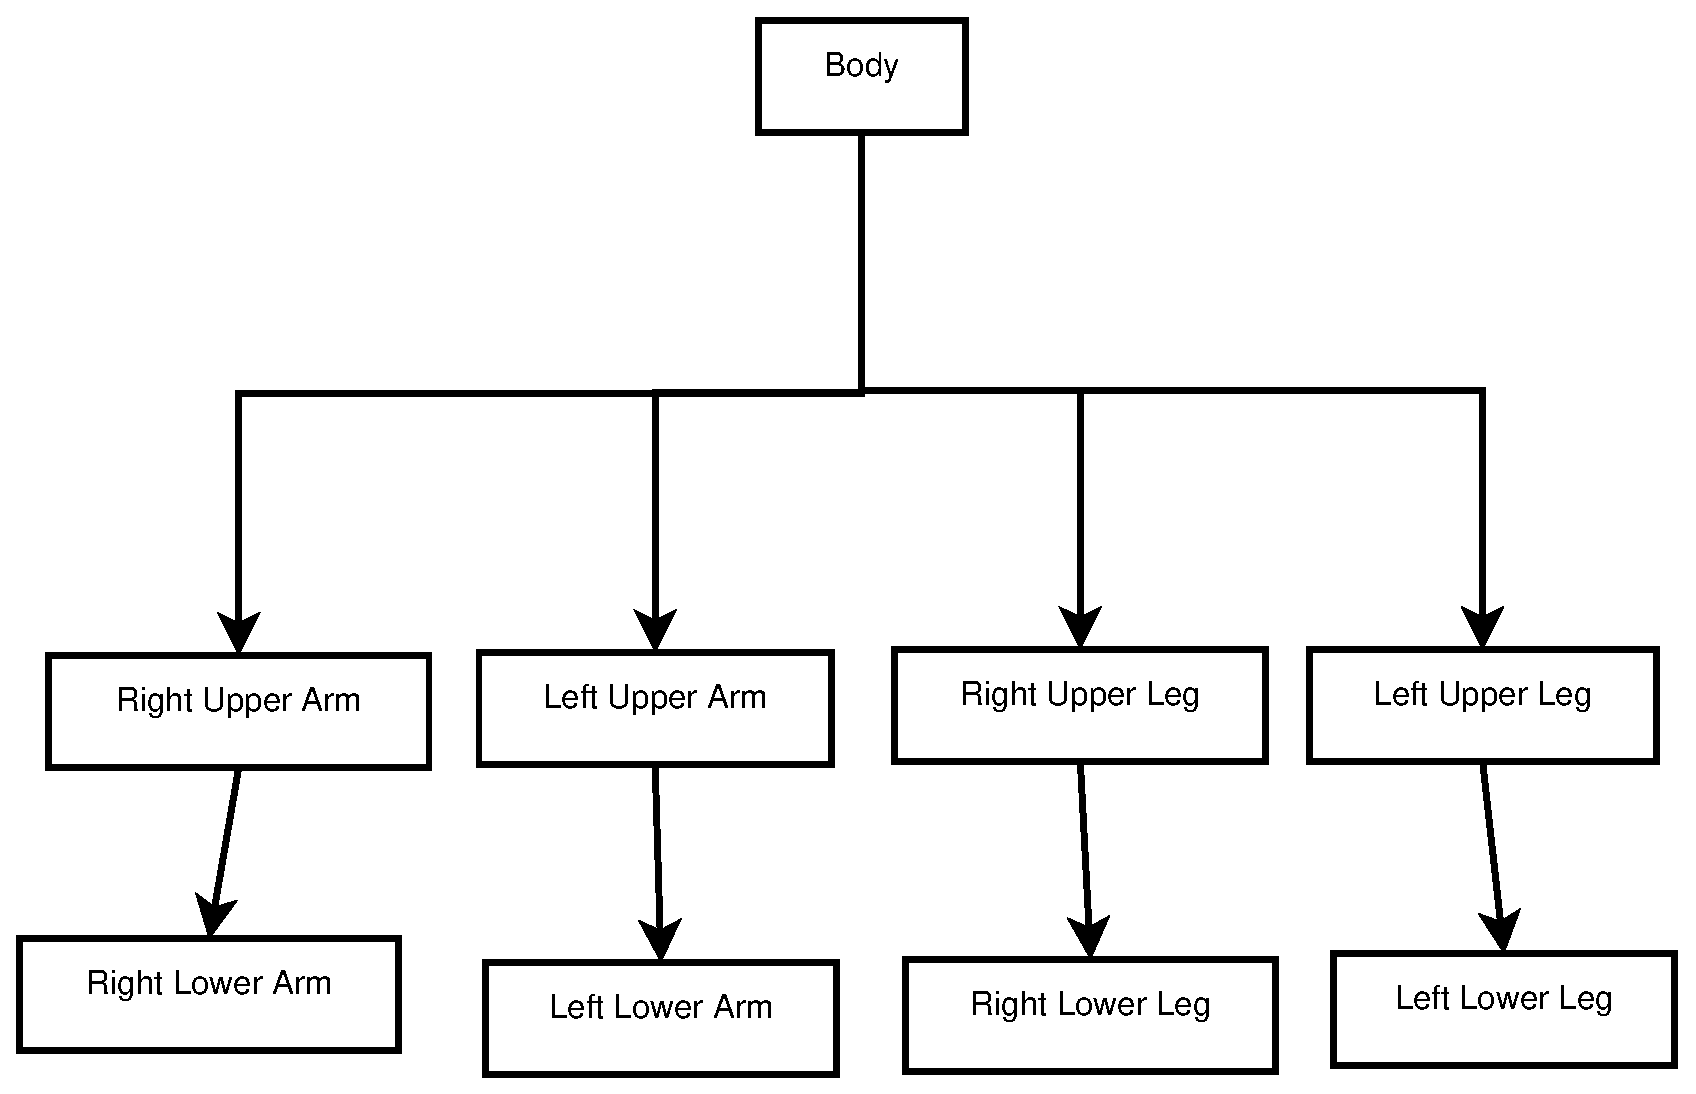
\includegraphics[width=\textwidth]{KinematicTree}
    \caption{This is some awesome thing.}
    \label{fig:tree2}
\end{figure}


\bibliography{ashwin_refs}{}
\addcontentsline{toc}{chapter}{REFERENCES}
\bibliographystyle{unsrt}
\end{document}
